\chapter{Description and implementation of attenuation}\label{C:attenuation}

%%%%%%%%%%%%%%%%%%%%%%%%%%%%%%%%%%%%%%%%%%%%%
% The visco-elastic rheology and memory variables
%%%%%%%%%%%%%%%%%%%%%%%%%%%%%%%%%%%%%%%%%%%%%

\section{The visco-elastic rheology and memory variables}\label{S:attenuation}

The numerical implementation of attenuation is largely motivated by
technical convenience and not so much by the true physics of seismic
wave attenuation in the interior of the Earth. In our analysis we closely follows Robertsson et al. (1994),
but introduce some modifications that facilitate the construction of constant-$Q$ models.\\
Assume that $\sigma, C$ and $\epsilon$ are representative of some
particular components of $\s{\sigma}, \w{C}$ and $\s{\epsilon}$,
respectively. Then a scalar version of the stress-strain relation is
given by
\begin{equation}\label{E:setup16}
\dot{\sigma}(t) = (\dot{C}*\dot{\epsilon})(t) =
\int\limits_{-\infty}^{\infty} \dot{C}(t-t') \dot{\epsilon}(t')\,
dt'\,.
\end{equation}
The spatial dependence has been omitted for brevity. As already
discussed, we choose the stress relaxation function or elastic
tensor component $C$ to be that of a superposition of $N$ standard
linear solids, weighted by coefficients $D_p$ ($p=1, ..., N)$, i.e.,
\begin{equation}\label{E:setup17}
C(t) := C_r \left[ 1- \sum_{p=1}^{N} D_p\, \left( 1-
\frac{\tau_{\epsilon p}}{\tau_{\sigma p}}\right)\,e^{-t/\tau_{\sigma
p}}\right] \, H(t)\,,
\end{equation}
where $\tau_{\epsilon p}$ and $\tau_{\sigma p}$ are the strain and
stress relaxation times of the $p$th standard linear solid,
respectively. The symbol $H$ denotes the Heaviside function and
$C_r$ is the relaxed modulus. Equation (\ref{E:setup17}) is very
general so that  different sets of relaxation times can give almost
the same relaxation function $C(t)$. To reduce this subjectively
undesirable non-uniqueness we limit the number of free parameters.
Following the $\tau$-method introduced by Blanch et al. (1995) we
determine the relaxation times $\tau_{\epsilon p}$ by defining a
dimensionless variable $\tau$ through
\begin{equation}\label{E:setup18}
\tau := \frac{\tau_{\epsilon p}}{\tau_{\sigma p}} -1\, .
\end{equation}
This gives
\begin{equation}\label{E:setup19}
C(t) = C_r \left[ 1+\tau\, \sum_{p=1}^{N} D_p\, e^{-t/\tau_{\sigma
p}} \right]\, H(t)\,.
\end{equation}
Differentiating (\ref{E:setup19}) with respect to $t$ and
introducing the result into equation (\ref{E:setup16}) yields
\begin{equation}\label{E:setup20}
\dot{\sigma}(t) = C_r (1+s\,\tau)\,\dot{\epsilon}(t) + C_r
\sum_{p=1}^{N} M_p\,,\quad s:=\sum_{p=1}^N D_p
\end{equation}
where the memory variables $M_p$ are defined by
\begin{equation}\label{E:setup21}
M_p := -\frac{D_p\,\tau}{\tau_{\sigma
p}}\,\int\limits_{-\infty}^{\infty} e^{-(t-t')/\tau_{\sigma p}}\,
H(t-t')\,\dot{\epsilon}(t')\, dt'\,.
\end{equation}
The differentiation of (\ref{E:setup21}) with respect to time yields
a set of first-order differential equations for the memory
variables:
\begin{equation}\label{E:setup22}
\dot{M_p} = -\frac{D_p\,\tau}{\tau_{\sigma p}} \, \dot{\epsilon} -
\frac{1}{\tau_{\sigma p}}\, M_p\,.
\end{equation}
Anelasticity can thus be modelled by simultaneously sloving the
momentum equation, a modified stress-strain relation and a set of
$N$ ordinary differential equations for the memory variables $M_p$.
The memory variables are formally independent of the elastic
parameter $C_r$. This formulation, proposed by Moczo \& Kristek
(2005), gives more accurate results in the case of strong attenuation heterogeneities than the classical formulation by Robertsson et al. (1994).\\
Generalising equations (\ref{E:setup20}) and (\ref{E:setup22}) to
the case of a three-dimensional and anisotropic medium with radial
symmetry axis is straightforward. The component-wise stress-strain
relation in the absence of dissipation is given by the following set
of equations:
\begin{subequations}\label{E:setup32}
\begin{align}
\sigma_{rr}&=(\kappa-2\mu/3)(\epsilon_{rr}+\epsilon_{\theta\theta}+\epsilon_{\phi\phi})+2\mu\epsilon_{rr}+c(\epsilon_{\theta\theta}+\epsilon_{\phi\phi})\\
\sigma_{\phi\phi}&=(\kappa-2\mu/3)(\epsilon_{rr}+\epsilon_{\theta\theta}+\epsilon_{\phi\phi})+2\mu\epsilon_{\phi\phi}+c\epsilon_{rr}+a(\epsilon_{\theta\theta}+\epsilon_{\phi\phi})\\
\sigma_{\theta\theta}&=(\kappa-2\mu/3)(\epsilon_{rr}+\epsilon_{\theta\theta}+\epsilon_{\phi\phi})+2\mu\epsilon_{\theta\theta}+c\epsilon_{rr}+a(\epsilon_{\theta\theta}+\epsilon_{\phi\phi})\\
\sigma_{r\phi}&=2(\mu+b)\epsilon_{r\phi}\\
\sigma_{r\theta}&=2(\mu+b)\epsilon_{r\theta}\\
\sigma_{\phi\theta}&=2\mu\epsilon_{\phi\theta}
\end{align}
\end{subequations}
We introduced the bulk modulus $\kappa=\lambda+\frac{2}{3}\mu$
because it is $-$ in contrast to the Lam\'{e} parameter $\lambda$ $-$
physically interpretable.\footnote{\textsf{There is, to the best of
my knowledge, no physical interpretation of $\lambda$. The
unphysical nature of this parameter becomes most apparent through
the fact that the $Q$ factor associated with $\lambda$, denoted by
$Q_\lambda$, can be negative for positive $Q_\mu$ and $Q_\kappa$.
Thus, if there were a physical process, e.g. an elastic wave, that
depended only on $\lambda$ and $\rho$, then this process would go
hand in hand with a continuously growing elastic energy.}} The
transition to the dissipative medium is now made by analogy:
\begin{subequations}\label{E:setup33}
\begin{align}
\dot{\sigma}_{rr}&=\left[\kappa_r
(1+s_\kappa \tau_\kappa)-\frac{2}{3}\mu_r(1+s_\mu \tau_\mu)\right]\,(\dot{\epsilon}_{rr}+\dot{\epsilon}_{\theta\theta}+\dot{\epsilon}_{\phi\phi})+2\mu_r(1+s_\mu\,\tau_\mu)\dot{\epsilon}_{rr}+c(\dot{\epsilon}_{\theta\theta}+\dot{\epsilon}_{\phi\phi})\notag\\
&+\kappa_r\sum_{p=1}^N \left(
K_{p}^{rr}+K_{p}^{\theta\theta}+K_{p}^{\phi\phi}\right)
-\frac{2}{3}\mu_r \sum_{p=1}^{N} \left(
M_p^{\theta\theta}+M_p^{\phi\phi} \right) + \frac{4}{3} \mu_r
\sum_{p=1}^{N} M_p^{rr}\\
\dot{\sigma}_{\phi\phi}&=\left[\kappa_r
(1+s_\kappa \tau_\kappa)-\frac{2}{3}\mu_r(1+s_\mu \tau_\mu)\right]\,(\dot{\epsilon}_{rr}+\dot{\epsilon}_{\theta\theta}+\dot{\epsilon}_{\phi\phi})+2\mu_r(1+s_\mu \tau_\mu)\dot{\epsilon}_{\phi\phi}+c\dot{\epsilon}_{rr}+a(\dot{\epsilon}_{\theta\theta}+\dot{\epsilon}_{\phi\phi})\notag\\
&+\kappa_r\sum_{p=1}^N \left(
K_{p}^{rr}+K_{p}^{\theta\theta}+K_{p}^{\phi\phi}\right)-\frac{2}{3}\mu_r
\sum_{p=1}^{N}
\left(M_p^{rr}+M_p^{\theta\theta}\right)+\frac{4}{3}\mu_r
\sum_{p=1}^{N} M_p^{\phi\phi}\\
\dot{\sigma}_{\theta\theta}&=\left[\kappa_r
(1+s_\kappa \tau_\kappa)-\frac{2}{3}\mu_r(1+s_\mu \tau_\mu)\right]\,(\dot{\epsilon}_{rr}+\dot{\epsilon}_{\theta\theta}+\dot{\epsilon}_{\phi\phi})+2\mu_r(1+s_\mu \tau_\mu)\dot{\epsilon}_{\theta\theta}+c\dot{\epsilon}_{rr}+a(\dot{\epsilon}_{\theta\theta}+\dot{\epsilon}_{\phi\phi})\notag\\
&+\kappa_r\sum_{p=1}^N \left(
K_{p}^{rr}+K_{p}^{\theta\theta}+K_{p}^{\phi\phi}\right)-\frac{2}{3}\mu_r
\sum_{p=1}^{N} \left(M_p^{rr}+M_p^{\phi\phi}\right)+\frac{4}{3}\mu_r
\sum_{p=1}^{N} M_p^{\theta\theta}\\
\dot{\sigma}_{r\phi}&=2\mu_r(1+s_\mu \tau_\mu)\dot{\epsilon}_{r\phi}+2b\dot{\epsilon}_{r\phi}+2\mu_r\sum_{p=1}^{N}
M_p^{r\phi}\\
\dot{\sigma}_{r\theta}&=2\mu_r(1+s_\mu \tau_\mu)\dot{\epsilon}_{r\theta}+2b\dot{\epsilon}_{r\phi}+2\mu_r\sum_{p=1}^{N}
M_p^{r\theta}\\
\dot{\sigma}_{\phi\theta}&=2\mu_r(1+s_\mu \tau_\mu)\dot{\epsilon}_{\phi\theta}+2\mu_r
\sum_{p=1}^{N} M_p^{\phi\theta}
\end{align}
\end{subequations}
For equations (\ref{E:setup33}) we assumed that the parameters $a,
b$ and $c$ are not involved in the dissipation of elastic energy.
The memory variables associated with $\mu$ $-$ denoted by $M_p^{ij}$
$-$ and the memory variables associated with $\kappa$ $-$ denoted by
$K_p^{ij}$ $-$ are governed by the first-order differential
equations
\begin{align}\label{E:setup34}
\dot{M}_p^{ij}&=-\frac{D_{p,\mu}\,\tau_\mu}{\tau_{\sigma p, \mu}}
\dot{\epsilon}_{ij} - \frac{1}{\tau_{\sigma p,\mu}} M_{p}^{ij}\\
\dot{K}_p^{ij}&=-\frac{D_{p,\kappa}\,\tau_\kappa}{\tau_{\sigma p, \kappa}}
\dot{\epsilon}_{ij} - \frac{1}{\tau_{\sigma p,\kappa}} K_{p}^{ij}
\end{align}
The above description of anelasticity is computationally inexpensive
compared to the spatial discretisation of the equations of motion
which account for the largest portion of the computational costs.

%%%%%%%%%%%%%%%%%%%%%%%%%%%%%%%%%%%%%%%%%%%%%
% Q and velocity dispersion
%%%%%%%%%%%%%%%%%%%%%%%%%%%%%%%%%%%%%%%%%%%%%

\section{$Q$ and phase velocity dispersion}

In seismology there has traditionally been more emphasis on the
quality factor Q than on particular stress or strain relaxation
functions. The definition of $Q$ is based on the definition of the
complex modulus
\begin{equation}\label{E:setup28}
\mathcal{C}(\nu) := \w{i}\,\nu\,\int_{0}^{\infty} C(t)\,e^{-\w{i}\nu
t}\, dt\,,
\end{equation}
with $\nu:=\omega+\w{i}\gamma$ and the damping factor $\gamma<0$. Then
\begin{equation}\label{E:setup29}
Q(\omega) :=
\frac{\frak{Re}\,\mathcal{C}(\omega)}{\frak{Im}\,\mathcal{C}(\omega)}\,.
\end{equation}
For our stress relaxation function defined in equation
(\ref{E:setup19}) we find
\begin{equation}\label{E:setup31a}
\mathcal{C}(\omega)=C_r + \w{i}\omega C_r\,\tau\,\sum_{p=1}^{N} \frac{D_p}{\w{i}\omega + \tau_{\sigma p}^{-1}}=A(\omega)+\w{i}\,B(\omega)\,,
\end{equation}
with the real and imaginary parts
\begin{equation}\label{E:setup31c}
A(\omega)=C_r\,\left[1+\tau\,\sum_{p=1}^{N} \frac{D_p\omega^2 \tau_{\sigma p}^2}{1+\omega^2 \tau_{\sigma p}^2}\right]\,,\quad B(\omega)=C_r\tau\,\sum_{p=1}^{N} \frac{D_p \omega \tau_{\sigma p}}{1+\omega^2 \tau_{\sigma p}^2}\,.
\end{equation}
Therefore, $Q$ is explicitly given by
\begin{equation}\label{E:setup31b}
Q(\omega) = \frac{ \left( 1+ \sum_{p=1}^{N} \frac{D_p\,\omega^2
\tau_{\sigma p}^2\tau}{1+\omega^2 \tau_{\sigma p}^2} \right)}{
\sum_{p=1}^{N} \left( \frac{D_p\,\omega \tau_{\sigma p}
\tau}{1+\omega^2\tau_{\sigma p}^2} \right)}\,.
\end{equation}
Visco-elastic dissipation implies phase velocity dispersion, where the phase velocity $v$ is defined by
\begin{equation}\label{E:setup32}
v=\frac{\omega}{\frak{Re}\,k}\,.
\end{equation}
The wave number is determined by the dispersion relation
\begin{equation}\label{E:setup33}
k^2=\frac{\omega^2 \rho}{\mathcal{C}}\,,
\end{equation}
which follows directly from the one-dimensional wave equation with a spatially invariable $C$. After some algebra, we find
\begin{equation}\label{E:setup34}
(\frak{Re}\,k)^2=\frac{1}{2}\,\rho\omega^2\,\frac{A+\sqrt{A^2+B^2}}{A^2+B^2}\,,
\end{equation}
and
\begin{equation}\label{E:setup35}
v^2=\frac{2\,(A^2+B^2)}{\rho\,(A+\sqrt{A^2+B^2})}\,.
\end{equation}

%%%%%%%%%%%%%%%%%%%%%%%%%%%%%%%%%%%%%%%%%%%%%
% Q and the loss of elastic energy
%%%%%%%%%%%%%%%%%%%%%%%%%%%%%%%%%%%%%%%%%%%%%

\section{$Q$ and the loss of elastic energy}

The quality factor $Q$ and its most common interpretation is closely related to the loss of elastic energy, that finds its most prominent expression in the reduction of the displacement amplitude, as the wave progresses in time and space. To see this, we first write the solution of the scalar wave equation in terms of the real and imaginary parts of the complex wave number $k=k_r+\w{i}\,k_i$:
\begin{equation}\label{E:Qintro027}
u(x,t)=u_0 e^{\w{i}\,(k_r x-\omega t)}\,e^{-k_i x}\,.
\end{equation}
Equation (\ref{E:Qintro027}) reveals that $k_i$ describes the amplitde reduction with increasing propagation distance. Let us now determine $k_i$ explicitly, first in terms of $A$ and $B$. For $k_i$ we find
\begin{equation}\label{E:Qintro028}
k_i^2=\frac{1}{2} \frac{\rho\omega^2}{A^2+B^2}\left( \sqrt{A^2+B^2}-A \right)\,.
\end{equation}
Working under the assumption that $Q$ is large, i.e. $B$ is small, we find the first-order expression
\begin{equation}\label{E:Qintro029}
k_i^2 \approx \frac{1}{4} \frac{\rho\omega^2 A Q^{-1}}{A^2+B^2}\,.
\end{equation}
Furthermore, for large $Q$, we have $v^2\approx A/\rho$, and equation (\ref{E:Qintro029}) simplifies to
\begin{equation}\label{E:Qintro030}
k_i = \frac{\omega}{2vQ}\,,
\end{equation}
where we replaced $\approx$ by $=$ for clarity in the following expressions. Based on equation (\ref{E:Qintro030}) we find that the amplitude reduction is proportional to $\exp\left(-\frac{\omega x}{2vQ}\right)$, and that the elastic energy reduction is proportional to  $\exp\left(-\frac{\omega x}{vQ}\right)$. Thus, by progressing from position $x$ to position $x+\lambda$, where $\lambda$ is the wavelength, the fractional energy loss is, correct to first order, given by
\begin{equation}\label{E:Qintro031}
\frac{E(x+\lambda)-E(x)}{E(x)}=-\frac{2\pi}{Q}\,.
\end{equation}
Equation (\ref{E:Qintro031}) can be interpreted as the definition of the \emph{spatial $Q$}. Alternatively, we may substitute $x=vt$, and then ask how the energy is reduced during one temporal osciallation cycle, i.e., as we progress from time $t$ to time $t+T$, where $T=\lambda v^{-1}$ is the period. Then we find, again correct to first order,
\begin{equation}\label{E:Qintro032}
\frac{E(t+T)-E(t)}{E(t)}=-\frac{2\pi}{Q}\,.
\end{equation}
This defines the \emph{temporal $Q$}.

%%%%%%%%%%%%%%%%%%%%%%%%%%%%%%%%%%%%%%%%%%%%%
% Q models
%%%%%%%%%%%%%%%%%%%%%%%%%%%%%%%%%%%%%%%%%%%%%

\section{Constructing constant-$Q$ models}

\subsection{Continuous case}

We are interested in constructing $Q$ models that are approximately independent of frequency for circular frequencies $\omega$ that are within the absorption band
\begin{equation}\label{E:Qconst001}
\tau_1 \ll \omega^{-1} \ll \tau_2\,,
\end{equation}
where $\tau_1$ and $\tau_2$ are stress-relaxation times that define the boundaries of the absorption band. Constructing such constant-$Q$ models means to find a set of stress-relaxation times $\tau_{\sigma p}$ and weights $D_p$ such that $Q(\omega)\approx \text{const}$ for $\omega$ satisfying (\ref{E:Qconst001}). This is a difficult undertaking, which requires a non-linear optimisation of equation (\ref{E:setup17}).\\
To facilitate our analysis, we make a detour via the case of a continuous distribution of standard-linear solids, i.e. we generalise equation (\ref{E:setup17}) to
\begin{equation}\label{E:Qconst002}
C(t)=C_r\,\left[1+\tau\,\int_{0}^{\infty} D(\tau_\sigma)\,e^{-t/\tau_\sigma}\,d\tau_\sigma \right]\,H(t)\,.
\end{equation}
The complex modulus is then
\begin{equation}\label{E:Qconst004}
\mathcal{C}(\omega)=A(\omega)+\w{i}B(\omega)\,,
\end{equation}
with
\begin{equation}\label{E:Qconst005}
A(\omega)=C_r\,\left[1+\tau\,\int_0^\infty \frac{\omega^2 \tau_\sigma^2}{1+\omega^2\tau_\sigma^2}\,D(\tau_\sigma)\,d\tau_\sigma \right]\,,\quad B(\omega)=C_r\,\left[\tau\,\int_0^\infty \frac{\omega\tau_\sigma}{1+\omega^2\tau_\sigma^2} D(\tau_\sigma)\,d\tau_\sigma   \right]\,.
\end{equation}
Choosing
\begin{equation}\label{E:Qconst006}
D(\tau_\sigma)=\begin{cases}
&\tau_\sigma^{-1}\,,\quad \text{for}\quad \tau_1\leq\tau_\sigma\leq\tau_2\notag\\
& 0\,,\quad \text{otherwise} \end{cases}\,,
\end{equation}
we obtain
\begin{align}\label{E:Qconst007}
A(\omega)&=C_r\,\left[1+\frac{1}{2}\tau\,\ln\left(\frac{1+\omega^2\tau_2^2}{1+\omega^2 \tau_1^2}  \right)\right]\,,\\
B(\omega)&=C_r\tau\,\left[\arctan(\omega\tau_2)-\arctan(\omega\tau_1) \right]\,.
\end{align}
For $\omega$ well within the absorption band, we obtain the useful approximations
\begin{equation}\label{E:Qconst008}
Q^{-1}\approx\frac{1}{2}\,\tau\pi = \text{const.}\,,
\end{equation}
and
\begin{equation}\label{E:Qconst009}
v\approx \sqrt{\frac{C_r}{\rho}} \left[1+\frac{1}{\pi Q}\,\ln(\omega\tau_2)\right]\,.
\end{equation}
As desired, $Q$ is approximately constant. Furthermore, the phase velocity increases with increasing frequency. This result implies that the weights of the relaxation mechanisms in the discrete case, $D_p$, should be proportional to $\tau_{\sigma p}^{-1}$. The parameter $\tau$ controls the numerical value of $Q$, and the relaxation times $\tau_{\sigma p}$ control the width of the absorption band. An example is shown in figure \ref{F:absorption_continuous}.
%====================================================================
\begin{center}
\begin{figure}
\center\scalebox{0.45}{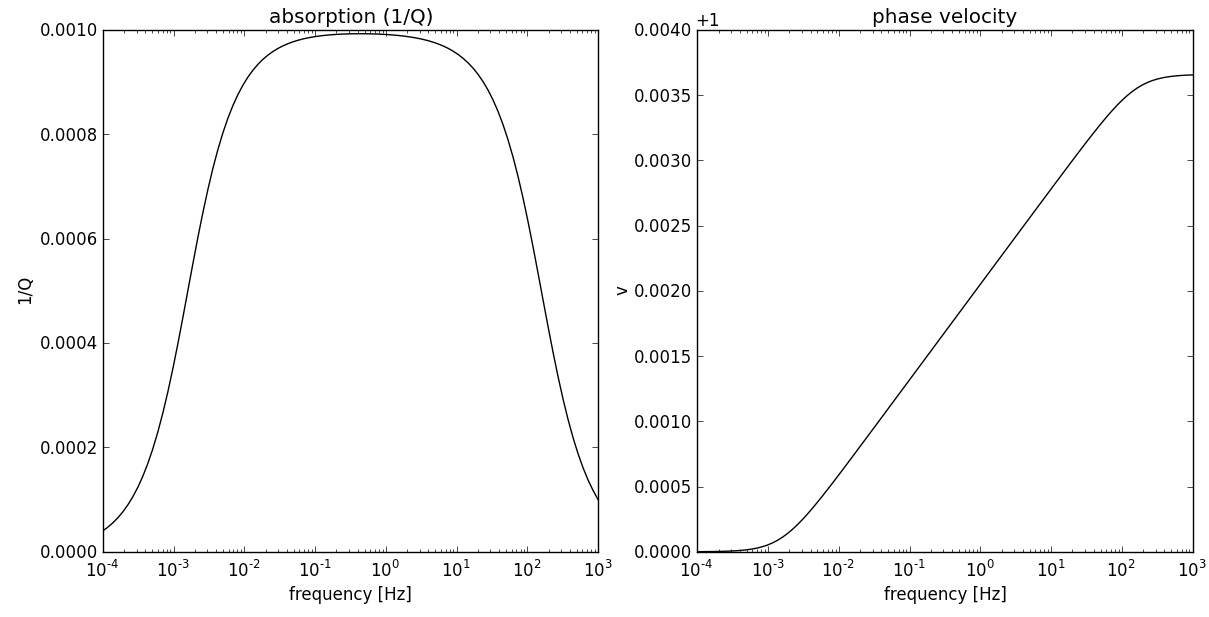
\includegraphics{Figures/absorption_band_continuous.jpg}} 
\caption{Example of a continuous absorption-band model with $Q=1000$, $\tau_1=1\cdot 10^{-3}$ s and $\tau_2=1\cdot 10^{2}$ s. The frequency-dependence of $Q^{-1}$ and the phase velocity $v$ are shown. This plot was produced using the Python tool \texttt{Q\_continuous.py} in the \texttt{TOOLS} directory.}\label{F:absorption_continuous}
\end{figure}
\end{center}
%====================================================================

\subsection{Discrete case}\label{S:Qdiscrete}

In the case of a discrete superposition of a finite number of relaxation mechanisms, the previous analysis is not sufficiently accurate because the frequency range considered is usually rather narrow. Therefore, we only take a few relaxation mechanisms (typically $2$ to $4$) with relaxation times $\tau_{\sigma p}$ and assign initial weights as $D_p=\tau_{\sigma p}$. Using a non-linear optimisation we then find optimal $\tau_{\sigma p}$ and $D_p$ such that
\begin{equation}\label{E:Qconst010}
\sum_{p=1}^{N} \frac{D_p \omega \tau_{\sigma p}}{1+\omega^2 \tau_{\sigma p}^2}=\frac{\pi}{2}\,,
\end{equation}
within the desired frequency band. For large $Q$, the relation between $Q$ and $\tau$ is then the same as for the continuous case:
\begin{equation}\label{E:Qconst011}
Q^{-1}\approx\frac{1}{2}\,\tau\pi \,.
\end{equation}
Figure \ref{F:absorption_discrete} shows an example.
%====================================================================
\begin{center}
\begin{figure}
\center\scalebox{0.45}{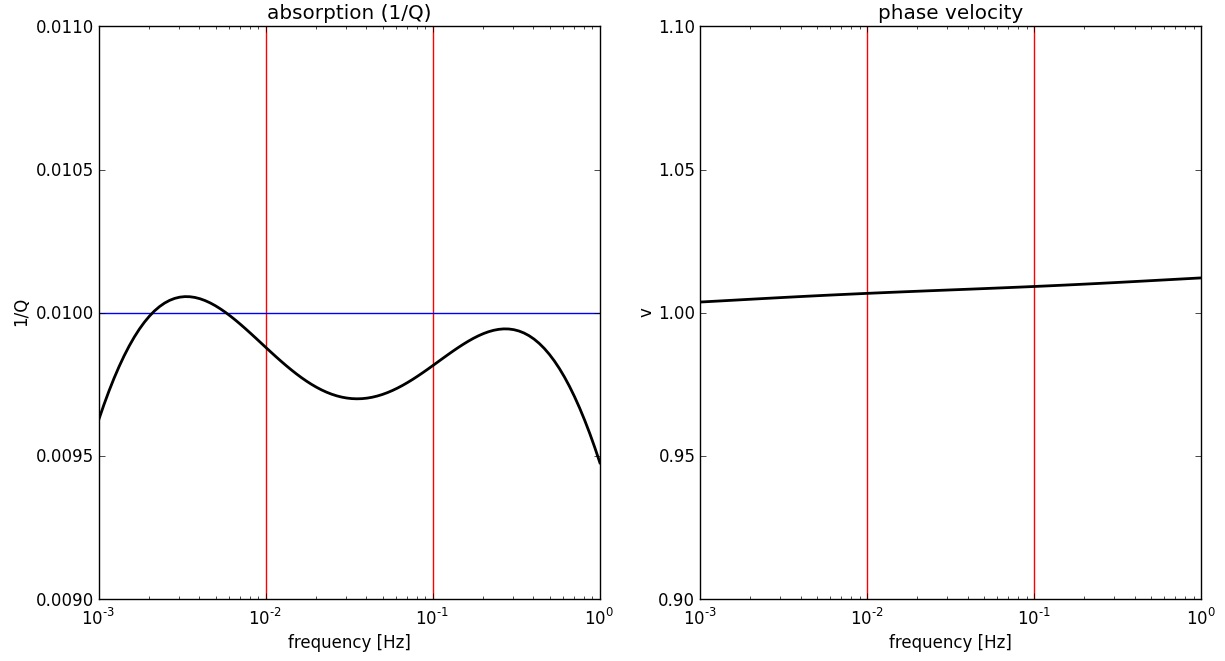
\includegraphics{Figures/absorption_band_discrete.jpg}} 
\caption{Example of a discrete absorption-band model with a constant target $Q=100$ in the frequency range $1\cdot 10^{-3}$-$1\cdot 10^{-2}$ Hz, which is indicated by red vertical lines. The number of relaxation mechanisms is $N=3$. This plot was produced using the Python tool \texttt{Q\_discrete.py} in the \texttt{TOOLS} directory.}\label{F:absorption_discrete}
\end{figure}
\end{center}
%====================================================================